%% lualatex tenuki30
\nonstopmode

\documentclass[11pt,a4paper]{ltjsarticle}
\usepackage{amsmath}
\usepackage{bm}
\usepackage{listings}
\usepackage{graphicx}
\usepackage{here}
\usepackage{listings,jvlisting}
\usepackage{threeparttable}
\usepackage{url}

\title{手抜きについて}
\author{手抜きチーム}
\date{2021年3月28日}

\begin{document}

\maketitle


手抜きはCSAプロトコルで対局を行うコンピュータ将棋プログラムです。開発者らが将棋プログラムの仕組みを理解するために作っています。 \\
リポジトリ:\url{https://github.com/hikaen2/tenuki-d}


\subsection*{名前の由来}
かっこいい名前が思いつかなかったため『手抜き』にしました。


\subsection*{特長}

\begin{itemize}
  \item 初段〜二段くらいの棋力
  \item αβ探索
  \item D言語で実装
%  \item 差分評価してません
%  \item 千日手チェックしてません
%  \item 詰将棋してません
%  \item ponderしてません
\end{itemize}


\subsection*{開発者}

鈴木太朗:自転車と合唱とEmacsが好きです。誰かdf-pn教えてください。Twitter: @hikaen2

玉川直樹:好きなコードはadd9です。将棋ウォーズ2段。Twitter: @Neakih\_kick


\section{今年の目標}

NNUEを理解する。


\section{使用ライブラリ}

\begin{itemize}
  \item 『どうたぬき』(tanuki- 第1回世界将棋AI 電竜戦バージョン)の評価関数ファイル nn.bin\footnote{\url{https://github.com/nodchip/tanuki-/releases/tag/tanuki-denryu1}}
\end{itemize}


\section{メモ:nn.binの構造について}

どうたぬきの評価関数ファイル nn.bin は64,217,066バイトある。
その内訳を表\ref{table1}に示す。
値はすべてリトルエンディアンで格納されている。

\begin{table}
  \footnotesize
  \centering
  \caption{どうたぬきのnn.binの内訳}
  \begin{tabular}{rlrrl}
    No. & 内容                       & 開始位置   & サイズ(バイト) & 備考 \\
    \hline
    1   & version                    & 0          & 4          & 0x7af32f16 \\
    2   & hash                       & 4          & 4          & 0x3e5aa6ee \\
    3   & size                       & 8          & 4          & 0x000000b2(architectureのサイズ. 可変) \\
    4   & architecture               & 12         & 178        & - \\
    5   & header                     & 190        & 4          & - \\
    6   & FeatureTransformer.biases  & 194        & 512        & $\vec{\bm{b}}_1$: int16\_tが256個 \\
    7   & FeatureTransformer.weights & 706        & 64,198,656 & $\bm{W}_1$: int16\_tが256\times 81\times 1548個 \\
    8   & header                     & 64,199,362 & 4          & - \\
    9   & HiddenLayer1.biases        & 64,199,366 & 128        & $\vec{\bm{b}}_2$: int32\_tが32個 \\
    10  & HiddenLayer1.weights       & 64,199,494 & 16,384     & $\bm{W}_2$: int8\_tが32\times 512個 \\
    11  & HiddenLayer2.biases        & 64,215,878 & 128        & $\vec{\bm{b}}_3$: int32\_tが32個 \\
    12  & HiddenLayer2.weights       & 64,216,006 & 1,024      & $\bm{W}_3$: int8\_tが32\times 32個 \\
    13  & OutputLayer.biases         & 64,217,030 & 4          & $\vec{\bm{b}}_4$: int32\_tが1個 \\
    14  & OutputLayer.weights        & 64,217,034 & 32         & $\bm{W}_4$: int8\_tが1\times 32個 \\
    \hline
        &                            &            & 合計: 64,217,066 &
  \end{tabular}
  \label{table1}
\end{table}

表\ref{table1}のNo.4: architectureには人間に可読な形式でニューラルネットワークの構造が書かれている。
どうたぬきの場合は

{
\small
\begin{verbatim}
Features=HalfKP(Friend)[125388->256x2],Network=AffineTransform[1<-32](ClippedReLU[32](
AffineTransform[32<-32](ClippedReLU[32](AffineTransform[32<-512](InputSlice[512(0:512)])))))
\end{verbatim}
}

\noindent
と書かれている。
この文字列の長さはニューラルネットワークの構造によって変わるので,その長さ(バイト数)がNo.3: sizeに格納されている。
どうたぬきの場合は0x000000b2 = 178である。

No.7: FeatureTransformer.weights ($\bm{W}_1$) は $256 \times 125388$ 行列である:

\[
  \bm{W}_1 =
  \left(
    \begin{array}{ccc}
      w_{1(0,0)}   & \ldots & w_{1(0,125387)} \\
      \vdots    & \ddots & \vdots \\
      w_{1(255,0)} & \ldots & w_{1(255,125387)}
    \end{array}
  \right)
\]

\noindent
この行列は125388次元の特徴ベクトルを256次元ベクトルに変換する。
ここで$125388 = 81 \times 1548$はKP(K:自玉とP:玉以外の駒 の組み合わせ)が取りうる場合の数である。
81はKの取りうる場合の数(玉が1一から9九まで。盤面のアドレスを図\ref{fig1}に示す),1548はPの取りうる場合の数(内訳を表\ref{table2}に示す)である。
この特徴ベクトルは駒のあるところが1,駒のないところが0になる二値ベクトルである。
将棋の駒は玉を除くと38枚あるので,特徴ベクトルは125388次元のうち38ヶ所だけが1で,のこりがすべて0のベクトルとなる。
特徴ベクトルの具体例については次節に記す。

$\bm{W}_1$はnn.binにcolumn-majorで格納されている。すなわち最初の値は$w_{(0,0)}$,次の値は$w_{(1,0)}$,… という順番で格納されている。
一方,後述する$\bm{W}_2$, $\bm{W}_3$, $\bm{W}_4$はrow-majorで格納されている。すなわち最初の値は$w_{(0,0)}$,次の値は$w_{(0,1)}$,… という順番で格納されている。
$\bm{W}_1$とそれ以外で格納順が異なることに注意されたい。

\begin{figure}
  \centering
  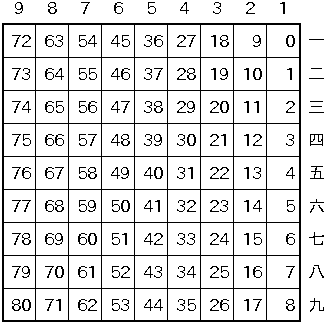
\includegraphics{fig/fig1.pdf}
  \caption{盤面のアドレス}
  \label{fig1}
\end{figure}


\begin{table}
  \footnotesize
  \centering
  \caption{Pの取りうる場合の数}
  \begin{threeparttable}
  \begin{tabular}{rlrrr}
    No. & 内容                            & 開始序数 & 場合の数 \\
    \hline
     1 & 味方の持駒の歩の0枚目~18枚目     &    0 & 19 \\
     2 & 相手の持駒の歩の0枚目~18枚目     &   19 & 19 \\
     3 & 味方の持駒の香の0枚目~4枚目      &   38 &  5 \\
     4 & 相手の持駒の香の0枚目~4枚目      &   43 &  5 \\
     5 & 味方の持駒の桂の0枚目~4枚目      &   48 &  5 \\
     6 & 相手の持駒の桂の0枚目~4枚目      &   53 &  5 \\
     7 & 味方の持駒の銀の0枚目~4枚目      &   58 &  5 \\
     8 & 相手の持駒の銀の0枚目~4枚目      &   63 &  5 \\
     9 & 味方の持駒の金の0枚目~4枚目      &   68 &  5 \\
    10 & 相手の持駒の金の0枚目~4枚目      &   73 &  5 \\
    11 & 味方の持駒の角の0枚目~2枚目      &   78 &  3 \\
    12 & 相手の持駒の角の0枚目~2枚目      &   81 &  3 \\
    13 & 味方の持駒の飛の0枚目~2枚目      &   84 &  3 \\
    14 & 相手の持駒の飛の0枚目~2枚目      &   87 &  3 \\
    15 & 味方の歩が1一〜9九にいる        &   90 & 81 \\
    16 & 相手の歩が1一〜9九にいる        &  171 & 81 \\
    17 & 味方の香が1一〜9九にいる        &  252 & 81 \\
    18 & 相手の香が1一〜9九にいる        &  333 & 81 \\
    19 & 味方の桂が1一〜9九にいる        &  414 & 81 \\
    20 & 相手の桂が1一〜9九にいる        &  495 & 81 \\
    21 & 味方の銀が1一〜9九にいる        &  576 & 81 \\
    22 & 相手の銀が1一〜9九にいる        &  657 & 81 \\
    23 & 味方の金\tnote{*} が1一〜9九にいる &  738 & 81 \\
    24 & 相手の金\tnote{*} が1一〜9九にいる &  819 & 81 \\
    25 & 味方の角が1一〜9九にいる        &  900 & 81 \\
    26 & 相手の角が1一〜9九にいる        &  981 & 81 \\
    27 & 味方の馬が1一〜9九にいる        & 1062 & 81 \\
    28 & 相手の馬が1一〜9九にいる        & 1143 & 81 \\
    29 & 味方の飛が1一〜9九にいる        & 1224 & 81 \\
    30 & 相手の飛が1一〜9九にいる        & 1305 & 81 \\
    31 & 味方の龍が1一〜9九にいる        & 1386 & 81 \\
    32 & 相手の龍が1一〜9九にいる        & 1467 & 81 \\
    \hline
       &                                   &      & 合計: 1548
  \end{tabular}
  \begin{tablenotes}
    \item[*] と・成香・成桂・成銀は金として扱う
  \end{tablenotes}
  \end{threeparttable}
  \label{table2}
\end{table}


No.6: FeatureTransformer.biases ($\vec{\bm{b}}_1$) は256次元ベクトルである:

\[
  \vec{\bm{b}}_1 =
  \left(
    \begin{array}{c}
      b_{1(0)}  \\
      \vdots \\
      b_{1(255)}
    \end{array}
  \right)
\]

\noindent
このベクトルは$\bm{W}_1$の出力である256個のニューロンに足すバイアスである。

$\bm{W}_1$にKPの125388次元の特徴ベクトル $\vec{\bm{x}}$ を掛けて,$\vec{\bm{b}}_1$を足すと,256次元のベクトル $\vec{\bm{y}}$ が得られる:

\[
  \underbrace{\left(
    \begin{array}{c}
      y_{0}   \\
      \vdots    \\
      y_{255} 
    \end{array}  
  \right)}_{\vec{\bm{y}}}
  =
  \underbrace{\left(
    \begin{array}{c}
      b_{1(0)}   \\
      \vdots    \\
      b_{1(255)} 
    \end{array}  
  \right)}_{\vec{\bm{b}}_1}
  +
  \underbrace{\left(
    \begin{array}{ccc}
      w_{1(0,0)}   & \ldots & w_{1(0,125387)} \\
      \vdots    & \ddots & \vdots \\
      w_{1(255,0)} & \ldots & w_{1(255,125387)}
    \end{array}
  \right)}_{\bm{W}_1}
  \times
  \underbrace{\left(
    \begin{array}{c}
      x_{0}   \\
      \vdots    \\
      x_{125387} 
    \end{array}  
  \right)}_{\vec{\bm{x}}}
\]

\noindent
この256次元ベクトル $\vec{\bm{y}}$ を先手分と後手分あわせて512次元にしたベクトルを$\vec{\bm{z}}_1$とする。
$\vec{\bm{z}}_1$を
No.10: HiddenLayer1.weights ($\bm{W}_2$ : $32 \times 512$ 行列) と
No.9: HiddenLayer1.biases ($\vec{\bm{b}}_2$ : 32次元ベクトル) に入力すると
32次元ベクトル$\vec{\bm{z}}_2$が得られる:

\[
  \underbrace{\left(
    \begin{array}{c}
      z_{2(0)}   \\
      \vdots    \\
      z_{2(31)} 
    \end{array}  
  \right)}_{\vec{\bm{z}}_2}
  =
  \underbrace{\left(
    \begin{array}{c}
      b_{2(0)}   \\
      \vdots    \\
      b_{2(31)} 
    \end{array}  
  \right)}_{\vec{\bm{b}}_2}
  +
  \underbrace{\left(
    \begin{array}{ccc}
      w_{2(0,0)}   & \ldots & w_{2(0,511)} \\
      \vdots    & \ddots & \vdots \\
      w_{2(31,0)} & \ldots & w_{2(31,511)}
    \end{array}
  \right)}_{\bm{W}_2}
  \times
  \sigma 
  \underbrace{\left(
    \begin{array}{c}
      z_{1(0)}   \\
      \vdots    \\
      z_{1(511)} 
    \end{array}  
  \right)}_{\vec{\bm{z}_1}}
\]

\noindent
ここで $\sigma$ はベクトルの各要素を0〜127の範囲にクリップする活性化関数 clipped ReLU である。
具体的には0以下の値は0にクリップする。127以上の値は127にクリップする。


次に $\vec{\bm{z}}_2$ を
No.12: HiddenLayer2.weights ($\bm{W}_3$ : $32 \times 32$ 行列) と
No.11: HiddenLayer2.biases ($\vec{\bm{b}}_3$ : 32次元ベクトル) に入力すると
32次元ベクトル$\vec{\bm{z}}_3$が得られる:


\[
  \underbrace{\left(
    \begin{array}{c}
      z_{3(0)}  \\
      \vdots    \\
      z_{3(31)} 
    \end{array}  
  \right)}_{\vec{\bm{z}}_3}
  =
  \underbrace{\left(
    \begin{array}{c}
      b_{3(0)}  \\
      \vdots    \\
      b_{3(31)} 
    \end{array}  
  \right)}_{\vec{\bm{b}}_3}
  +
  \underbrace{\left(
    \begin{array}{ccc}
      w_{3(0,0)}   & \ldots & w_{3(0,31)} \\
      \vdots       & \ddots & \vdots \\
      w_{3(31,0)}  & \ldots & w_{3(31,31)}
    \end{array}
  \right)}_{\bm{W}_3}
  \times
  \sigma 
  \underbrace{\left(
    \begin{array}{c}
      z_{2(0)}   \\
      \vdots    \\
      z_{2(31)} 
    \end{array}  
  \right)}_{\vec{\bm{z}_2}}
\]

\pagebreak
最後に $\vec{\bm{z}}_3$ を
No.14: OutputLayer.weights ($\bm{W}_4$ : $1 \times 32$ 行列) と
No.13: OutputLayer.biases ($\vec{\bm{b}}_4$ : 1次元ベクトル) に入力すると
1次元ベクトル$\vec{\bm{z}}_4$が得られる。これが評価値である:

\[
  \underbrace{\left(
    \begin{array}{c}
      z_{4(0)}
    \end{array}  
  \right)}_{\vec{\bm{z}}_4}
  =
  \underbrace{\left(
    \begin{array}{c}
      b_{4(0)}
    \end{array}  
  \right)}_{\vec{\bm{b}}_4}
  +
  \underbrace{\left(
    \begin{array}{ccc}
      w_{4(0,0)}   & \ldots & w_{4(0,31)} \\
    \end{array}
  \right)}_{\bm{W}_4}
  \times
  \sigma 
  \underbrace{\left(
    \begin{array}{c}
      z_{3(0)}   \\
      \vdots    \\
      z_{3(31)} 
    \end{array}  
  \right)}_{\vec{\bm{z}_3}}
\]


以上の計算を図に表すと図\ref{fig4}となる(バイアス $\vec{\bm{b}}_n$ と活性化関数 $\sigma$ の記載は省略している)。

以上の計算を行うサンプルプログラムを \url{https://github.com/hikaen2/nnue-test} に作成した(D言語)。



\begin{figure}
  \centering
  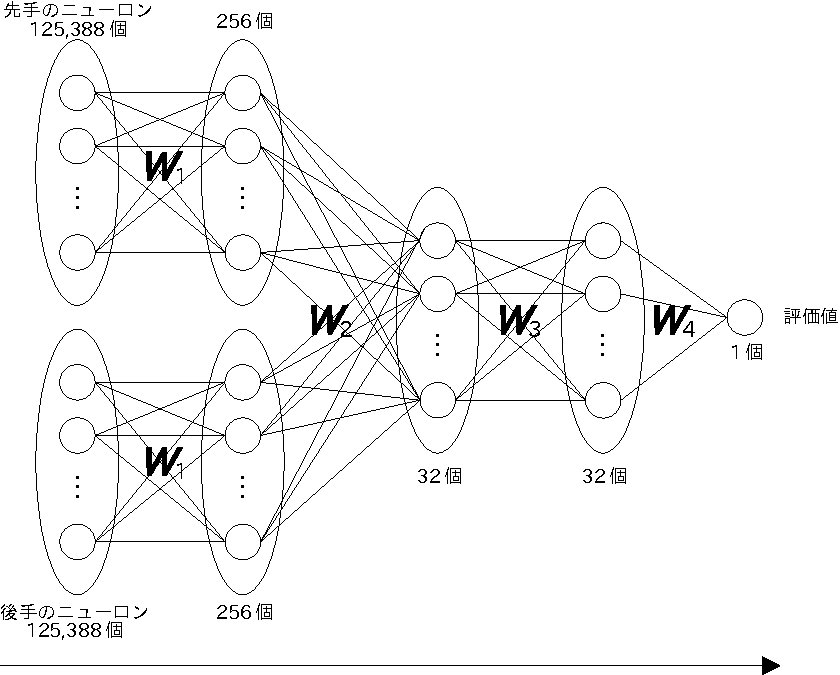
\includegraphics[width=12cm]{fig/fig4.pdf}
  \caption{ニューラルネットワークの図(先手の評価値を求めるとき)}
  \label{fig4}
\end{figure}




\subsection{特徴ベクトルの具体例}

\subsubsection*{例1}

以下の局面を考える。

\nopagebreak
\begin{figure}[H]
  \centering
  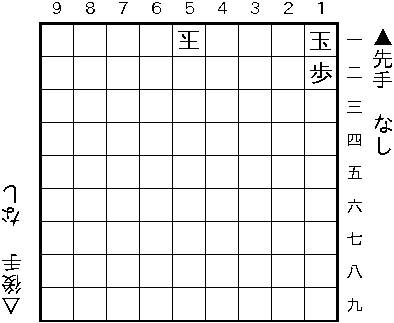
\includegraphics{fig/fig2.pdf}
\end{figure}

先手の特徴ベクトルを考える。
先手玉が1一にいる。図\ref{fig1}を見ると1一のアドレスは0なので,このときのKの序数は0になる。
1二に(先手から見て)味方の歩がいる。表\ref{table2}を見ると味方の歩の序数は90から始まっている。
これに1二のアドレスである1を足すと $90 + 1 = 91$ になり,1二にいる味方の歩を表現できる。
KとPを合わせると $0 \times 1548 + 91 = 91$ となる。
これは125388次元ベクトルの(0から数えて)91番目の要素に1を立てることを意味する。
したがって先手の特徴ベクトルはこのようになる:

\begin{eqnarray*}
    \vec{\bm{x}}
    =
    \begin{pmatrix}
        x_{0}  &=& 0 \\
        \vdots       \\
        x_{90} &=& 0 \\
        x_{91} &=& 1 \\
        x_{92} &=& 0 \\
        \vdots       \\
        x_{125387} &=& 0 \\
    \end{pmatrix}
\end{eqnarray*}

次に後手の特徴ベクトルを考える。
後手の特徴ベクトルを考えるときは盤面を180度回転する。
すると5一の後手玉は5九の位置にいることになる。図\ref{fig1}を見ると5九のアドレスは44なので,このときのKの序数は44になる。
つぎに1二に(後手から見て)相手方の歩がいる。これは盤面を180度回転すると9八の位置にいることになる。
表\ref{table2}を見ると相手方の歩の序数は171から始まっている。
これに9八のアドレスである79を足すと$171 + 79 = 250$になる。
KとPを合わせると$44 \times 1548 + 250 = 68362$となる。
これは125388次元ベクトルの(0から数えて)68362番目の要素に1を立てることを意味する。
したがって後手の特徴ベクトルはこのようになる:

\nopagebreak
\begin{eqnarray*}
    \vec{\bm{x}}
    =
    \begin{pmatrix}
        x_{0}  &=& 0 \\
        \vdots       \\
        x_{68361} &=& 0 \\
        x_{68362} &=& 1 \\
        x_{68363} &=& 0 \\
        \vdots       \\
        x_{125387} &=& 0 \\
    \end{pmatrix}
\end{eqnarray*}

\subsubsection*{例2}

以下の局面を考える。

\nopagebreak
\begin{figure}[H]
  \centering
  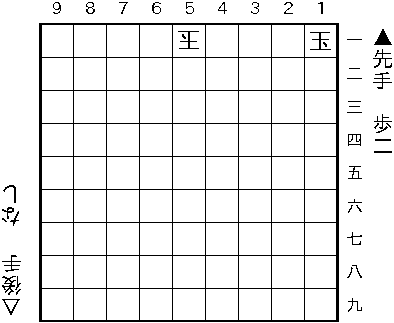
\includegraphics{fig/fig3.pdf}
\end{figure}

先手の特徴ベクトルを考える。
先手玉が1一にいる。図\ref{fig1}を見ると1一のアドレスは0なので,このときのKの序数は0になる。
味方の持ち駒に歩が2枚ある。
表\ref{table2}を見ると味方の持ち駒の歩の序数は0から始まっている。
そこで1枚目の歩は $0 + 1 = 1$ となる。2枚目の歩は $0 + 2 = 2$ となる:

\begin{eqnarray*}
    \vec{\bm{x}}
    =
    \begin{pmatrix}
        x_{0}  &=& 0 \\
        x_{1}  &=& 1 \\
        x_{2}  &=& 1 \\
        x_{3}  &=& 0 \\
        \vdots       \\
        x_{125387} &=& 0 \\
    \end{pmatrix}
\end{eqnarray*}




\section{私のためのQ\&A}

\begin{description}
  \item[Q1] NNUEはKPを入力とするニューラルネットワークということですか?
  \item[A1] そうです。厳密に言えばどうたぬきのNNUEについてはそうです。これはKP以外を入力とするNNUEも考えられるということです。
\end{description}

\begin{description}
  \item[Q2] なんでKPPより強いんですか?
  \item[A2] KPPの線形和より,KPの非線形和のほうが表現力があるということだと思います。
  言い換えると線形和がよほどよろしくないのかもしれません。
  たとえばカツカレーがおいしいのはカツがおいしくて,なおかつカレーがおいしいからと考えることもできますが,
  だからといっておいしいプリンをおいしいカレーに入れてもおいしくなるとは限らないということだと思います。
\end{description}

\begin{description}
  \item[Q3] 線形和・非線形和ってなんですか?
  \item[A3] 雑な理解として,線形和はとりあえず全部足したやつだと思っています。非線形和はとりあえず全部足したやつじゃない足し方をしたやつだと思っています。
\end{description}

\begin{description}
  \item[Q4] ベクトルってなんですか?
  \item[A4] プログラマとしては雑な理解として配列だと思っています。だから125388次元のベクトルは125388要素の配列だと思っています。
\end{description}

\begin{description}
  \item[Q5] 行列ってなんですか?
  \item[A5] 2次元配列だと思っています。
\end{description}

\begin{description}
  \item[Q6] バイアス ($\vec{\bm{b}}$) ってなんですか?
  \item[A6] 1次関数で言うところの切片だと思っています。つまり $y = ax + b$ の $b$にあたるものだと思っています。
\end{description}

\begin{description}
  \item[Q7] 線形代数はなにが線形なのですか?
  \item[A7] 雑な理解でいうと,ベクトルを行列によって変換したときの変換され具合が線形(1次関数によって計算される)なのだと思います。
  たとえば図形を行列で変形すると,どの座標の点も一様に変形されます。突然図形がぐにゃぐにゃになったりはしないということです。
\end{description}

\begin{description}
  \item[Q8] NNUEのニューラルネットワークの学習ってどうやるんですか?
  \item[A8] わかりません。これから調べます。
\end{description}


\section{参考文献}

\begin{itemize}
  \item 那須 悠, 高速に差分計算可能なニューラルネットワーク型将棋評価関数, \url{https://www.apply.computer-shogi.org/wcsc28/appeal/the_end_of_genesis_T.N.K.evolution_turbo_type_D/nnue.pdf}
\end{itemize}


\end{document}
